% !TeX spellcheck = en_US
\documentclass[a4paper,fleqn,11pt]{article}

% header
%% Packages 

% Styling TOC
\usepackage{tocloft}
\setlength\cftaftertoctitleskip{1cm}
\usepackage[nottoc]{tocbibind}

% Mathe Packages
\usepackage{amsmath,amssymb,epsfig,amsthm,amsfonts,bbm,textcomp}

% Grafiken
\usepackage[font=normalsize,aboveskip=0pt,belowskip=0pt,labelfont=bf]{caption}
\captionsetup{justification=centering,singlelinecheck=false}
\usepackage[edges]{forest}
\usepackage{tikz}
\usetikzlibrary{arrows,intersections,decorations.pathreplacing}
%\usetikzlibrary{angles,quotes}
\usepackage[utf8]{inputenc}
\usepackage[T1]{fontenc}
\usepackage{lmodern}
\usepackage[english]{babel}

% Seiten Layout
\usepackage{float} 				
\usepackage[top=3cm,bottom=3cm,left=3cm,right=3cm,a4paper]{geometry}  
\usepackage[onehalfspacing]{setspace}
\usepackage{color}
\usepackage{enumitem}

% Fussnoten
\usepackage[flushmargin,hang]{footmisc}
\usepackage{listings}
\usepackage[hyphens]{url}
\usepackage[hidelinks]{hyperref}


% Tabellen
\usepackage{longtable} 			% Lange, mehrseitige Tabelle
\usepackage{tabularx}
\usepackage{array,hhline}
\usepackage{booktabs}			% Linien zwischen Zeilen 
\usepackage{multirow}			% Verknüpfte Zellen über Zeilen hinweg
\usepackage{dcolumn}			% Erlaubt variable Orientierung am Decimalpunkt innerhalb einer Zelle
\usepackage{siunitx}

% References
\usepackage{natbib}






\begin{document}

% title page
%
% header

\pagenumbering{Roman}

\title{\huge Forecasting Swiss Exports using Bayesian \\Forecast Reconciliation}

\author[$\dagger$]{Florian Eckert}
\author[$\ddagger$]{Rob J. Hyndman}
\author[$\ddagger$]{Anastasios Panagiotelis}
\affil[$\dagger$]{\small KOF Swiss Economic Institute, ETH Zurich}
\affil[$\ddagger$]{\small Department of Econometrics and Business Statistics, Monash University}
\date{July 2019}

\maketitle
\begin{abstract}
\noindent This paper conducts an extensive forecasting study on 13,118 time series measuring Swiss goods exports, grouped hierarchically by export destination and product category.  We apply existing state of the art methods in forecast reconciliation and introduce a novel Bayesian reconciliation framework. This approach allows for explicit estimation of reconciliation biases, leading to several innovations: Prior judgment can be used to assign weights to specific forecasts and the occurrence of negative reconciled forecasts can be ruled out. Overall we find strong evidence that in addition to producing coherent forecasts, reconciliation also leads to improvements in forecast accuracy.

\noindent \textbf{JEL Classification:} C32, C53, E17\\
\noindent \textbf{Keywords}: Hierarchical Forecasting, Bayesian Forecast Reconciliation, Swiss Exports, Optimal Forecast Combination.
\end{abstract}
\clearpage




% table of contents
%\tableofcontents

%\clearpage

%\listoffigures
%\listoftables

%\clearpage

\pagenumbering{arabic}

			




% 2. Model	
\section{Introduction}
\label{sec:model}

Example of a hierarchy with $k = 3$ levels, $m = 13$ series in total and $q = 9$ series at the bottom of the hierarchy.\\

\begin{figure}[H]
	\centering
	\begin{forest}
	before packing={
		forked edges,
	}
		[{$Y_0$}
			 [{$Y_{01}$}
		 		[{$Y_{011}$}]
				[{$Y_{012}$}]
		 		[{$Y_{012}$}]
		 	]
			 [{$Y_{02}$}
		 		[{$Y_{021}$}]
				[{$Y_{022}$}]
		 		[{$Y_{023}$}]
		 	]
			 [{$Y_{03}$}
				[{$Y_{031}$}]
				[{$Y_{032}$}]
				[{$Y_{033}$}]
			]
		]
	\end{forest}
\vspace{0.5cm}
	\caption{Simple Example Hierarchy}
\end{figure}

If we define $Y_t = [Y_0, Y_{01}, Y_{02}, \hdots, Y_{033}]'$ to be an ($m \times 1$) vector of top-down stacked observations from all levels, it must hold at each point in time $t$ that
\begin{align}
Y_t &= S Y_{k,t}
\end{align}
where $Y_{k,t}$ is a ($q \times 1$) vector containing the observations at level $k$, the bottom of the hierarchy, and $S$ is an ($m \times q$) aggregation matrix. For the above example, $S$ has to be constructed in the following way.
\begin{align*} S &=
\begin{bmatrix}
\ 1 & 1 & 1 & 1 & 1 & 1 & 1 & 1 & 1\ \ \\
\ 1 & 1 & 1 & 0 & 0 & 0 & 0 & 0 & 0\ \ \\
\ 0 & 0 & 0 & 1 & 1 & 1 & 0 & 0 & 0\ \ \\
\ 0 & 0 & 0 & 0 & 0 & 0 & 1 & 1 & 1\ \ \\
\ 1 & 0 & 0 & 0 & 0 & 0 & 0 & 0 & 0\ \ \\
\ 0 & 1 & 0 & 0 & 0 & 0 & 0 & 0 & 0\ \ \\
  &   &   &   & \vdots &   &   &   &   \\
\ 0 & 0 & 0 & 0 & 0 & 0 & 0 & 0 & 1\ \ 
\end{bmatrix}
\end{align*}
For the forecasts to be consistent and additive, they usually have to be estimated either top-down or bottom-up. However, there are benefits to forecasting all series in the hierarchy. It might be that different models provide better fits, varying information sets are available, or judgment predictions have to be used. As a result of this, the different levels of the forecasted hierarchy usually cannot be aggregated consistently. In order to reconcile forecasts at each level of the hierarchy, \cite{Hyndman2011} show that optimal predictions at the bottom level can be obtained using the following regression approach.
\begin{align}
Y_t(h) &= S\beta_{h} + e_t(h)
\end{align}
where $Y_t(h)$ is an ($m \times 1$) vector containing the h-periods-ahead forecasts at time $t$ for each level in the hierarchy. $\beta_{h}$ represents the optimal predictions at the bottom level that minimize the deviations between the individual forecasts and the consistent hierarchy. The reconciliation error term $e_t(h)$ follows a normal distribution with mean 0 and covariance matrix $\Sigma_h$. There is obviously a high level of heteroskedasticity in the error terms, which is why $\beta_h$ has to be estimated using generalized least squares. The optimal point forecasts result therefore from the following weighted least squares regression.
\begin{align}
\label{eq:reg}
\beta_{h} &= \left(S'\Sigma_h^{-1}S \right)^{-1} S'\Sigma_h^{-1}Y_t(h)
\end{align}
Intuitively, $\beta_h$ minimizes the reconciliation error, which is the squared distance between the actual and reconciled forecasts. As a result of the weighting matrix, forecasts with a higher prediction error receive less weight in the regression.\\


\section{Bayesian Forecast Reconciliation}
\subsection{Proposition}
Since every forecast horizon is reconciled independently, the time subscripts are dropped from now on to simplify notation. It is assumed that we have $n$ samples from the predictive distribution of each of the $m$ predictions. Therefore, $Y_{i}$ denotes a vector length $m$ that contains a draw $i$ from the predictive distribution of all forecasts, where $i = 1,\hdots, n$. The unobservable error term consists of two components, a prediction error $e_{i}$ and a fixed effect $\alpha$. The latter is a vector of length $m$ and can be interpreted as containing the reconciliation errors that are specific to each forecasted variable. In other terms, $\alpha$ is the difference between the unreconciled forecast mean $\hat{Y}$ and the reconciled forecast mean $\tilde{Y}$. Furthermore, there is no common intercept by design. When all predictors are zero, no bottom-level forecasts are aggregated and the expected response should therefore be zero as well. Because the slope line passes through the origin, the reconciliation errors also do not necessarily sum to zero. The following regression equation can then be used to estimate $\alpha$ and $\beta$.
\begin{align}
Y_{i} &= \alpha + S\beta + e_{i}
\end{align}
where $e$ follows a normal distribution with mean zero and variance $\Sigma$. An error-components model of this form is quite frequently used in panel data regressions. Since the aggregation matrix $S$ is fixed, the reconciliation error is uncorrelated with the explanatory variables. It is therefore possible to treat the reconciliation errors as random effects and to omit $\alpha$ from the above regression. The optimal forecasts at the bottom level are then still estimated consistently. 

Estimating the reconciliation errors explicitly as a fixed effect has several advantages, but proves to be rather tricky. A standard technique in panel models is to get rid of the fixed effect by demeaning the data or taking first differences. If there is a sufficient number of observations, the fixed effects can then be retrieved by subtracting the fitted values from the responses. This is not possible here because there is no variation in the regressor $S$. Another approach would be to include a dummy for each variable to account for the fixed effects. However, this is unfeasible too because it leads to perfect multicollinearity in the explanatory variables.

\begin{figure}[H]
\label{jacksonpollock}
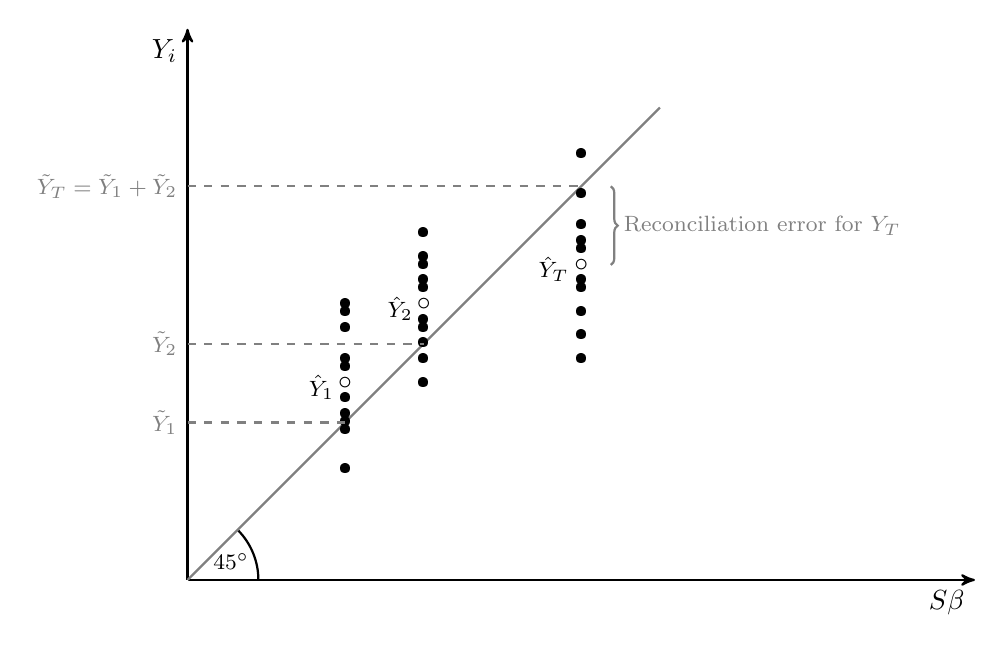
\begin{tikzpicture}[
    thick,
    >=stealth',
    dot/.style = {
      draw,
      fill = white,
      circle,
      inner sep = 0pt,
      minimum size = 4pt
    }
  ]
    \coordinate (O) at (0,0);
    \draw (0,0)+(0:0.9) arc(0:45:0.9);
    \node at (22.5:0.6) {\footnotesize $45^\circ$};
    \draw[->] (0,0) -- (0,7) coordinate[label = {below left:$Y_{i}$}] (ymax);
    \draw[->] (0,0) -- (10,0) coordinate[label = {below left:$S \beta$}] (xmax);
    \draw[gray] (0,0) -- (6,6);
    \foreach \Point in {(2,1.4), (2,1.9), (2,2), (2,2.1), (2,2.3),
                      (2,2.7), (2,2.8), (2,3.2), (2,3.4), (2,3.5)} \node at \Point {\textbullet};
    \foreach \Point in {(3,2.5), (3,2.8), (3,3), (3,3.2), (3,3.3),
                      (3,3.7), (3,3.8), (3,4), (3,4.1), (3,4.4)} \node at \Point {\textbullet};
    \foreach \Point in {(5,2.8), (5,3.1), (5,3.4), (5,3.7), (5,3.8),
                      (5,4.2), (5,4.3), (5,4.5), (5,4.9), (5,5.4)} \node at \Point {\textbullet};    

    \node [label = {[shift={(-0.35,-0.55)}] \footnotesize $\hat{Y}_T$}] at (5,4) {$\circ$};
    \node [label = {[shift={(-0.3,-0.55)}] \footnotesize $\hat{Y}_2$}] at (3,3.5) {$\circ$};
    \node [label = {[shift={(-0.3,-0.55)}] \footnotesize $\hat{Y}_1$}] at (2,2.5) {$\circ$};
    
    \draw[gray,dashed] (0,5) node[left]{\footnotesize $\tilde{Y}_T = \tilde{Y}_1 + \tilde{Y}_2$} -- (5,5);
    \draw[gray,dashed] (0,3) node[left]{\footnotesize $\tilde{Y}_2$} -- (3,3);    
    \draw[gray,dashed] (0,2) node[left]{\footnotesize $\tilde{Y}_1$} -- (2,2); 

    \draw[gray,decoration={brace,raise=5pt},decorate]
  (5.2,5) -- node[right=6pt] {\footnotesize Reconciliation error for $Y_T$} (5.2,4);
    
\end{tikzpicture}
\caption{Graphical Representation of a Reconciliation Regression.}
\end{figure}

A convenient solution to this identification problem comes from Bayesian econometrics. There are several other fields, where identification is achieved by means of informative priors. In structural vector auto-regressions, the structural coefficient matrices can be identified through prior assumptions about the sign of shocks \citep{Baumeister2015}. In dynamic factor models, different rotations of latent factors and loadings are observationally equivalent. The factors can be identified through prior restrictions on the factor loadings \citep{Bai2015}.

In Bayesian statistics, data is considered to be fixed and parameters are treated as random variables. The researcher has a prior belief about the distribution of the parameters in a model. After observing the data, this prior belief is combined with the likelihood according to Bayes' theorem in order to obtain the posterior distribution of the parameters. This principle can be applied to $\alpha$, $\beta$ and $\Sigma$ in the reconciliation regression. The consistent bottom-level forecasts $\beta$ follow a normal distribution with mean $b$ and covariance $B$. The reconciliation errors $\alpha$ are also distributed normally with mean $a$ and covariance $A$. The prediction errors follow a normal distribution with mean zero and variance $\Sigma$. The aggregation matrix $S$ and the sample of unreconciled forecasts $Y$ are believed to be fixed.
\begin{align}
f(\alpha, \beta, \Sigma\ |\ S,Y) \propto f(Y,S\ |\ \alpha, \beta, \Sigma) \times f(\alpha, \beta, \Sigma)
\end{align}
In other words, the posterior distribution of the bottom-level forecasts is proportional to the likelihood (of the hierarchy to be consistent) times the prior distribution of the bottom-level forecasts. We have little prior knowledge about the reconciled bottom-level forecasts $\beta$ and the predictive distribution $\Sigma$. However, we may have some prior belief about the reconciliation errors because we trust some forecasting models more than others. This could be due to better data availability, better forecasting performance in the past or subjective judgment of the forecaster. A sufficiently narrow prior for $\alpha$ allows the identification of the model parameters.\\




\subsection{Estimation}
In order to approximate the distribution of $Y_t(h)$, we draw $n$ h-periods-ahead-predictions $Y_i$, with $i = 1, \hdots, n$, from their forecasted distributions. This is equivalent to solving a seemingly unrelated regression using generalized least squares. Following \cite{Greenberg2008}, the likelihood function for the data is given by 
\begin{align*}
f(Y,S\ |\ \alpha,\beta,\Sigma) \propto \frac{1}{|\Sigma|}\exp\left[\frac{1}{2} \sum_i (Y_i - \alpha - S\beta)'\Sigma^{-1}(Y_i - \alpha - S\beta)\right]
\end{align*}
and the posterior distribution is accordingly given by
\begin{align*}
f(\alpha,\beta,\Sigma\ |\ Y,S) & \propto \frac{1}{|\Sigma|^{n/2}}\exp\left[-\frac{1}{2} \sum_i (Y_i - \alpha - S\beta)'\Sigma^{-1}(Y_i - \alpha - S\beta)\right] \\
&\times \exp \left[-\frac{1}{2}(\alpha - a_0)'A_0^{-1}(\alpha - a_0)\right] \\
&\times \exp \left[-\frac{1}{2}(\beta - b_0)'B_0^{-1}(\beta - b_0)\right] \\
&\times \frac{1}{|\Sigma|(v_0 - m - 1)} \exp \left[-\frac{1}{2} tr(R_0^{-1}\Sigma^{-1}) \right]
\end{align*}
We are interested in the marginal distribution of $\alpha$, $\beta$ and $\Sigma$. This can be achieved by approximating the joint posterior distribution through Gibbs sampling from the conditional distributions and then averaging the samples. See for instance \cite{Kim1999} (...) for derivation. First some random starting values for the parameters are chosen. Afterwards, the following steps are repeated until convergence:

\begin{enumerate}
\item \textbf{Draw $\alpha$ conditional on $\beta,\Sigma,Y,S$}\\
The fixed effects $\alpha$ can be obtained from a regression of $Y_i - S\beta$ on an identity matrix. The conditional posterior distribution for $\alpha$ is given by
\begin{align}
\alpha\ |\ \beta,\Sigma,Y,S &\sim N(a_1,A_1)
\end{align}
where
\begin{align*}
A_1 &= \left(\sum_i \Sigma^{-1} + A_0^{-1}\right)^{-1} = \left(n\Sigma^{-1} + A_0^{-1} \right)^{-1}\\
a_1 &= A_1 \left(\sum_i \Sigma^{-1} (Y_i - S\beta) + A_0^{-1}a_0\right)
\end{align*}
The prior mean $a_0$ should be set to zero and the prior covariance $A_0$ should be a diagonal matrix. The entries on the diagonal should be lower for forecasts that the researcher is more confident in. Entries that correspond to uncertain forecasts can be set higher. Perhaps a reasonable prior can be derived from the level of aggregation that the forecast is in. Different weighting schemes might be tested and conclusions can be drawn from the forecast combination literature, such as \cite{Cesur2016} or \cite{Brooks2001}.\\

\item \textbf{Draw $\beta$ conditional on $\alpha,\Sigma,Y,S$}\\
The slope coefficients $\beta$ can be obtained from a regression of $Y_i - \alpha$ on $S$. The conditional posterior distribution for $\beta$ is given by
\begin{align}
\beta\ |\ \alpha,\Sigma,Y,S &\sim N(b_1,B_1)
\end{align}
where
\begin{align*}
B_1 &= \left(\sum_i S'\Sigma^{-1}S + B_0^{-1}\right)^{-1} = \left(nS'\Sigma^{-1}S + B_0^{-1} \right)^{-1}\\
b_1 &= B_1 \left(\sum_i S'\Sigma^{-1} (Y_i - \alpha) + B_0^{-1}b_0\right)
\end{align*}
Unless we have some reason to believe otherwise, the priors $b_0$ and $B_0$ should be chosen as uninformative as possible. Prior belief on the divergence between the initial and the reconciled forecasts should be incorporated in the prior on $\alpha$. \\

\item \textbf{Draw $\Sigma$ conditional on $\alpha,\beta,Y,S$}\\
$\Sigma$ is a diagonal matrix since the $n$ draws from the predictive distribution come from different models and the approximated densities are generated independently. Because the off-diagonal elements are zero, it could also be seen as a weighted least squares regression. This resembles the alternative estimator \#3 for the coherency errors in \cite{Wickramasuriya2015}. Each entry $\sigma_{i}$ on the diagonal can therefore be drawn equation-by-equation from an inverse Gamma distribution.
\begin{align}
\sigma_{i}\ |\ \alpha,\beta,Y,S \sim IG(v_1/2,d_1/2)
\end{align}
where
\begin{align*}
v_1 &= v_0 + n\\
d_1 &= d_0 + \sum_i e_i'e_i
\end{align*}
where $e_i = Y_i - \alpha - S \beta$.\\

\item \textbf{Draw $\tilde{Y}$ conditional on $\alpha,\Sigma,\beta,S$}\\
We can also generate the predictive distribution (in the fitted value senses) for $\tilde{Y}$, the predictive density of $Y$. \cite{Percy1992} has shown that an analytic solution is difficult to calculate and it is far easier to draw samples from the joint posterior distribution of the parameters and then generate the predicted values of $Y$ conditional on the data.
\begin{align}
\tilde{Y}\ |\ \alpha,\beta,\Sigma,S \sim N(S\beta,\Sigma)
\end{align}
Convergence of the Gibbs sampler can be checked using the recursive mean of the chains. After convergence is achieved, a sufficiently large number of these draws are saved.
\end{enumerate}

\noindent The mean of the hierarchically consistent forecasts can then be computed using discrete statistics on the saved draws from the posterior.\\

\subsection{Prior Selection}
As noted before, the priors for the parameters should be as diffuse as possible with the exception of $A_0$, the prior variance of the fixed effects. There are several outcomes, depending on the information content of the prior.
\begin{itemize}
    \item\textbf{Diffuse prior}. Setting the prior variance of $\alpha$ close to infinity assumes that we have absolutely no knowledge about the reconciliation errors. As a result, the parameters cannot be uniquely identified and the Gibbs sampler does not converge. [Proof: Where is the boundary between diffuse and vague?]
    \item \textbf{Vague prior}. The prior variance of $\alpha$ can be set such that each entry is the same and reasonably low. This implies that we have some prior knowledge that the reconciliation errors are distributed around zero. As a result, $\beta$ reduces to the OLS estimate in \cite{Hyndman2011}. [Proof]
    \item \textbf{Informed prior}. The prior variance of $\alpha$ can also reflect prior knowledge. A high value on the diagonal of $A_0$ implies a belief that the reconciliation error is larger, whereas a small value implies a belief that the reconciliation error should be small. A natural choice for $A_0$ is a matrix with the corresponding variances of the prediction errors on the diagonal, which leads to the GLS estimate for $\beta$ in \cite{Hyndman2016}. [Proof]. Other possibilities for the prior variance could be the number of series at each node or manually setting the prior variance on specific reconciliation errors to zero. 
\end{itemize}

\clearpage

\section{Simulation Exercise}

Simulate hierarchies of various sizes, levels and time series properties and compare benchmark performance / forecasting accuracy with other methods such as
\begin{itemize}
    \item Top-Down Approach
    \item Bottom-Up Approach
    \item Middle-Out Approach
    \item GLS Reconciliation \cite{Hyndman2011}
    \item Minimum Trace Reconciliation \cite{Wickramasuriya2015}
    \item Alternative Weighting Matrices
    \item No Reconciliation\\
\end{itemize}

What happens if we have forecasts that do not follow a normal distribution? An example from my own experience: Swiss imports are driven quite heavily by imports of airplanes and it is uncertain when they arrive, e.g. forecasts are bimodal.

\clearpage

\section{Empirical Application}
\subsection{Data}
We use a comprehensive dataset of Swiss foreign trade in goods. For both exports and imports, it contains the nominal value in Swiss francs of goods traded with 245 countries and dependent territories. They are aggreg The goods are categorized according to the economic sector, following a national nomenclature covering 14 main groups and 272 subgroups. The hierarchy is unbalanced, meaning that certain goods categories are available more disaggregated than others. This results in a hierarchy with up to 5 levels. The 14 main groups are the following:
\begin{enumerate}[itemsep=-1ex,partopsep=1ex,parsep=1ex]
    \item Forestry and agricultural products, fisheries
    \item Energy source
    \item Textiles, clothing, shoes
    \item Paper, stationery and graphical products
    \item Leather, rubber, plastics 
    \item Products of the chemical and pharmaceutical industry
    \item Stones and earth
    \item Metals
    \item Machines, appliances, electronics
    \item Vehicles
    \item Precision instruments, clocks and watches and jewellery  
    \item Various goods such as music instruments, home furnishings, toys, sports equipment
    \item Precious metals, precious and semi-precious stones
    \item Works of art and antiques
\end{enumerate}
Because of the geographical and the categorical dimension, there is no unique hierarchical structure. Following \cite{Hyndman2016}, these time series can therefore be thought of as a grouped time series. There are 63'516 time series with non-zero entries in total, 35'602 for the export hierarchy and 27'914 for the import hierarchy. The time series are available in monthly frequency from 1989 on and are not adjusted for working days or seasonality. The data is collected by the Swiss Federal Customs Administration\footnote{\url{https://www.ezv.admin.ch/ezv/en/home/topics/swiss-foreign-trade-statistics.html}} and made available in a machine-friendly data format only on basis of a subscription.\\


\subsection{Results}
Repeat comparison from simulation exercise, construct export and import hierarchies by geographical region, countries and product categories. As a by-product, there could a visualization in the spirit of the MIT Trade Atlas\footnote{\url{https://atlas.media.mit.edu/en/visualize/tree_map/hs92/export/ltu/all/show/2016/ }} be developed.\\

Results from running hts on the data, using the average across the root mean squared errors and mean absolute percentage errors of all series.\\
\begin{table}[H]
\centering
\caption{Forecast Accuracy by Standard Aggregation Methods}
\small
\begin{tabularx}{\textwidth}{Xcclcclcclcc}
\toprule
& \multicolumn{2}{c}{Overall} & & \multicolumn{2}{c}{2003-2007} & & \multicolumn{2}{c}{2008-2012} & & \multicolumn{2}{c}{2013-2018}\\
\cmidrule{2-3} \cmidrule{5-6} \cmidrule{8-9} \cmidrule{11-12}
& \scriptsize{MAPE} & \scriptsize{RMSE} & & \scriptsize{MAPE} & \scriptsize{RMSE} & & \scriptsize{MAPE} & \scriptsize{RMSE} & & \scriptsize{MAPE} & \scriptsize{RMSE}\\ 
\midrule
Bottom-up &  &  &&  & && & && & \\ 
\quad \scriptsize{ETS} & 2.3 & 2.3  && 2.3 & 2.3 && 2.3 & 2.3 && 2.3 & 2.3\\ 
\quad \scriptsize{ARIMA} & 2.3 & 2.3  && 2.3 & 2.3 && 2.3 & 2.3 && 2.3 & 2.3\\
\addlinespace
Middle-out &  &  &&  & && & && & \\ 
\quad \scriptsize{ETS} & 2.3 & 2.3  && 2.3 & 2.3 && 2.3 & 2.3 && 2.3 & 2.3\\ 
\quad \scriptsize{ARIMA} & 2.3 & 2.3  && 2.3 & 2.3 && 2.3 & 2.3 && 2.3 & 2.3\\
\addlinespace
\multicolumn{3}{l}{Top-down (Gross-Sohl A)} &&  & && & && & \\ 
\quad \scriptsize{ETS} & 2.3 & 2.3  && 2.3 & 2.3 && 2.3 & 2.3 && 2.3 & 2.3\\ 
\quad \scriptsize{ARIMA} & 2.3 & 2.3  && 2.3 & 2.3 && 2.3 & 2.3 && 2.3 & 2.3\\
\addlinespace
\multicolumn{3}{l}{Top-down (Gross-Sohl F)} &&  & && & && & \\ 
\quad \scriptsize{ETS} & 2.3 & 2.3  && 2.3 & 2.3 && 2.3 & 2.3 && 2.3 & 2.3\\ 
\quad \scriptsize{ARIMA} & 2.3 & 2.3  && 2.3 & 2.3 && 2.3 & 2.3 && 2.3 & 2.3\\
\addlinespace
\multicolumn{3}{l}{Top-down (Forecast Proportions)} &&  & && & && & \\ 
\quad \scriptsize{ETS} & 2.3 & 2.3  && 2.3 & 2.3 && 2.3 & 2.3 && 2.3 & 2.3\\ 
\quad \scriptsize{ARIMA} & 2.3 & 2.3  && 2.3 & 2.3 && 2.3 & 2.3 && 2.3 & 2.3\\
\bottomrule
\end{tabularx}
\end{table}

Using optimal forecast combination with different weighting schemes:\\
\begin{table}[H]
\centering
\caption{Forecast Accuracy by Optimal Forecast Combination Weights}
\small
\begin{tabularx}{\textwidth}{Xcclcclcclcc}
\toprule
& \multicolumn{2}{c}{Overall} & & \multicolumn{2}{c}{2003-2007} & & \multicolumn{2}{c}{2008-2012} & & \multicolumn{2}{c}{2013-2018}\\
\cmidrule{2-3} \cmidrule{5-6} \cmidrule{8-9} \cmidrule{11-12}
& \scriptsize{MAPE} & \scriptsize{RMSE} & & \scriptsize{MAPE} & \scriptsize{RMSE} & & \scriptsize{MAPE} & \scriptsize{RMSE} & & \scriptsize{MAPE} & \scriptsize{RMSE}\\ 
\midrule
\multicolumn{3}{l}{OLS (unweighted combination) } &&  & && & && & \\ 
\quad \scriptsize{ETS} & 2.3 & 2.3  && 2.3 & 2.3 && 2.3 & 2.3 && 2.3 & 2.3\\ 
\quad \scriptsize{ARIMA} & 2.3 & 2.3  && 2.3 & 2.3 && 2.3 & 2.3 && 2.3 & 2.3\\
\addlinespace
\multicolumn{3}{l}{WLS (forecast variance weights) } &&  & && & && & \\ 
\quad \scriptsize{ETS} & 2.3 & 2.3  && 2.3 & 2.3 && 2.3 & 2.3 && 2.3 & 2.3\\ 
\quad \scriptsize{ARIMA} & 2.3 & 2.3  && 2.3 & 2.3 && 2.3 & 2.3 && 2.3 & 2.3\\
\addlinespace
\multicolumn{3}{l}{MinT (full covariance weights) } &&  & && & && & \\ 
\quad \scriptsize{ETS} & 2.3 & 2.3  && 2.3 & 2.3 && 2.3 & 2.3 && 2.3 & 2.3\\ 
\quad \scriptsize{ARIMA} & 2.3 & 2.3  && 2.3 & 2.3 && 2.3 & 2.3 && 2.3 & 2.3\\
\addlinespace
\multicolumn{3}{l}{nseries (numer of series at each node)} &&  & && & && & \\ 
\quad \scriptsize{ETS} & 2.3 & 2.3  && 2.3 & 2.3 && 2.3 & 2.3 && 2.3 & 2.3\\ 
\quad \scriptsize{ARIMA} & 2.3 & 2.3  && 2.3 & 2.3 && 2.3 & 2.3 && 2.3 & 2.3\\
\bottomrule
\end{tabularx}
\end{table}

\ \\

Results from Bayesian estimation.. In addition, it might be interesting to look at forecast errors for different regional/categorical aggregates:
\begin{table}[H]
\centering
\caption{Forecast Accuracy by Regional and Categorical Aggregates}
\small
\begin{tabularx}{\textwidth}{Xcclcclcclcc}
\toprule
& \multicolumn{2}{c}{Overall} & & \multicolumn{2}{c}{2003-2007} & & \multicolumn{2}{c}{2008-2012} & & \multicolumn{2}{c}{2013-2018}\\
\cmidrule{2-3} \cmidrule{5-6} \cmidrule{8-9} \cmidrule{11-12}
& \scriptsize{MAPE} & \scriptsize{RMSE} & & \scriptsize{MAPE} & \scriptsize{RMSE} & & \scriptsize{MAPE} & \scriptsize{RMSE} & & \scriptsize{MAPE} & \scriptsize{RMSE}\\ 
\midrule
\multicolumn{3}{l}{OLS (unweighted combination) } &&  & && & && & \\ 
\quad \scriptsize{ETS} & 2.3 & 2.3  && 2.3 & 2.3 && 2.3 & 2.3 && 2.3 & 2.3\\ 
\quad \scriptsize{ARIMA} & 2.3 & 2.3  && 2.3 & 2.3 && 2.3 & 2.3 && 2.3 & 2.3\\ 
\bottomrule
\end{tabularx}
\end{table}



\clearpage

\section{Conclusion}







\clearpage

% bibliography
\pagenumbering{Roman}
\setcounter{page}{3}
\bibliography{library}
\bibliographystyle{apalike}

\clearpage


% appendix

\appendix
\section{Appendix}


\subsection{Robustness}
\label{sec:robust}

\begin{figure}[H]
	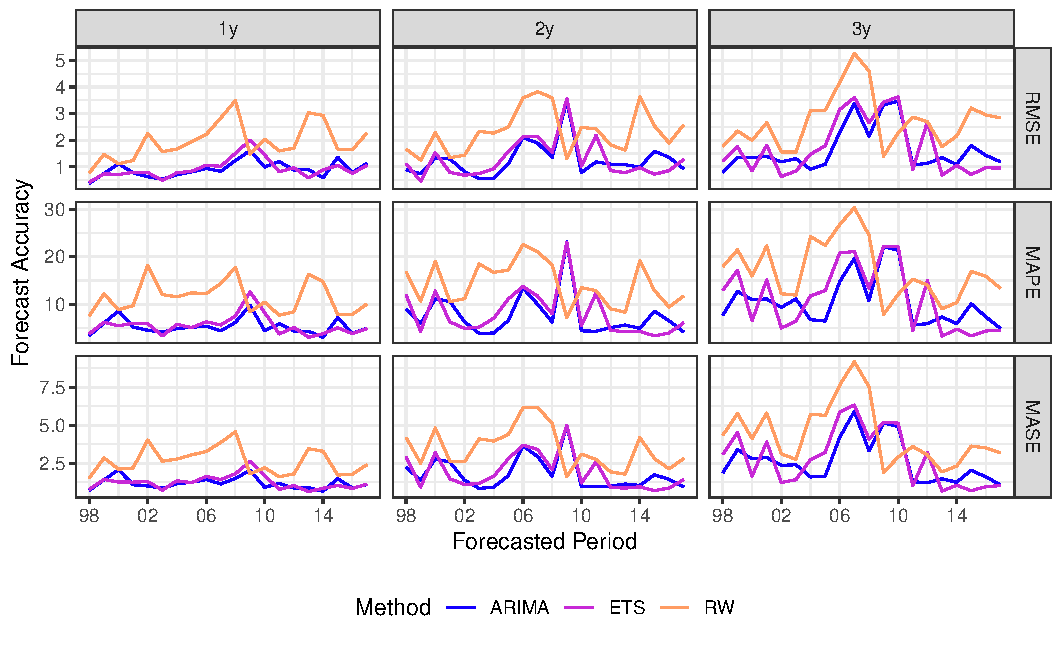
\includegraphics[width=\textwidth]{fig/fig_eval_methods_top}
	\caption{Accuracy of Forecasting Methods at the Top Level}
\end{figure}

\begin{figure}[H]
	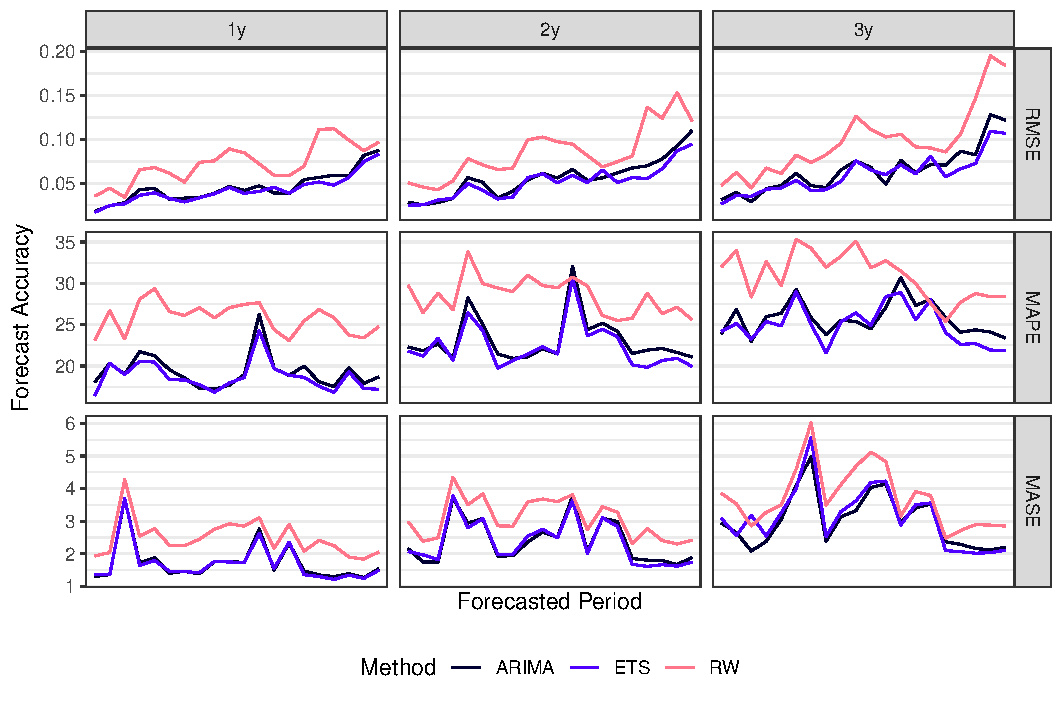
\includegraphics[width=\textwidth]{fig/fig_eval_methods_bottom}
	\caption{Accuracy of Forecasting Methods at the Bottom Level}
\end{figure}


\subsection{Data}
\label{sec:data}
The data is compiled by the Swiss Federal Customs Administration\footnote{\url{https://www.ezv.admin.ch/ezv/en/home/topics/swiss-foreign-trade-statistics.html}} and made available in a machine-friendly format on basis of a subscription.\\
% table with goods categories
\begin{small}
\begin{longtable}{p{2.5cm}p{11.5cm}}
\caption{Tariff Numbers and Descriptions of Goods}\\
\toprule
\normalsize{Tariff Number} & \normalsize{Description}\\
\midrule
\endfirsthead
\multicolumn{2}{@{}l}{\ldots continued}\\
\toprule
\normalsize{Tariff Number} & \normalsize{Description}\\  
\midrule
\endhead
\bottomrule
\multicolumn{2}{r@{}}{continued \ldots}\\
\endfoot
\bottomrule
\endlastfoot
	01	&	Forestry and agricultural products, fisheries	\\
\enskip	01.1	&	Food, beverages and tobacco	\\
\enskip	01.2	&	Feeding stuffs for animals	\\
\enskip	01.3	&	Live animals	\\
\enskip	01.4	&	Horticultural products	\\
\enskip	01.5	&	Forestry products (not firewood)	\\
\enskip	01.6	&	Products for commercial/industrial further processing such as oils, fats, starches, plants and vegetable parts, etc.	\\
\midrule
	02	&	Energy source	\\
\enskip	02.1	&	Solid combustibles	\\
\enskip	02.2	&	Petroleum and distillates	\\
\enskip	02.3	&	Gas	\\
\enskip	02.4	&	Electrical energy	\\
\midrule
	03	&	Textiles, clothing, shoes	\\
\enskip	03.1	&	Textiles	\\
\enskip	03.2	&	Articles of apparel and clothing	\\
\enskip	03.3	&	Shoes, parts and accessories	\\
\midrule
	04	&	Paper, articles of paper and and products of the printing industry	\\
\enskip	04.1	&	Basic materials for paper production, such as cellulose and cellulose fibre and paper and carton waste	\\
\enskip	04.2	&	Paper and carton in rolls, strips or sheets	\\
\enskip	04.3	&	Goods from paper or carton	\\
\enskip	04.4	&	Products of the printing industry	\\
\midrule
	05	&	Leather, rubber, plastics	\\
\enskip	05.1	&	Leather	\\
\enskip	05.2	&	Rubber	\\
\enskip	05.3	&	Plastics	\\
\midrule
	06	&	Products of the chemical and pharmaceutical industry	\\
\enskip	06.1	&	Chemical raw materials, basic materials and unformed plastics	\\
\enskip	06.2	&	Chemical end products, vitamins, diagnostic products, including active substances	\\
\midrule
	07	&	Stones and earth	\\
\enskip	07.1	&	Mineral raw materials and basic products	\\
\enskip	07.2	&	Goods from stone and cement	\\
\enskip	07.3	&	Ceramic wares	\\
\enskip	07.4	&	Glass	\\
\midrule
	08	&	Metals	\\
\enskip	08.1	&	Iron and steel	\\
\enskip	08.2	&	Non-ferrous metals	\\
\enskip	08.3	&	Metal goods	\\
\midrule
	09	&	Machines, appliances, electronics	\\
\enskip	09.1	&	Industrial machinery	\\
\enskip	09.2	&	Agricultural machines	\\
\enskip	09.3	&	Household appliances	\\
\enskip	09.4	&	Office machines	\\
\enskip	09.5	&	Electrical and electronic industry appliances and devices	\\
\enskip	09.6	&	Military equipment	\\
\midrule
	10	&	Vehicles	\\
\enskip	10.1	&	Road vehicles	\\
\enskip	10.2	&	Railed vehicles	\\
\enskip	10.3	&	Air- and spacecraft	\\
\enskip	10.4	&	Watercraft	\\
\midrule
	11	&	Precision instruments, clocks and watches and jewellery	\\
\enskip	11.1	&	Precision instruments and equipment	\\
\enskip	11.2	&	Watches	\\
\enskip	11.3	&	Jewellery and household goods made from precious metals	\\
\midrule
	12	&	Various goods such as music instruments, home furnishings, toys, sports equipment, etc.	\\
\enskip	12.1	&	Exposed film	\\
\enskip	12.2	&	Music instruments	\\
\enskip	12.3	&	Home furnishings	\\
\enskip	12.4	&	Toys and sports equipment	\\
\enskip	12.5	&	Stationery goods	\\
\enskip	12.6	&	Various goods such as umbrellas, neon signs, festive articles, brushes, lighters, pipes, etc.	\\
\midrule
	13	&	Precious metals, precious and semi-precious stones	\\
\enskip	13.1	&	Precious and semi-precious stones	\\
\enskip	13.2	&	Precious metals (including gold and silver bars from 1.1.2012)	\\
\midrule
	14	&	Works of art and antiques	\\
\enskip	14.1	&	Works of art	\\
\enskip	14.2	&	Antiques and collectors' items	\\
\end{longtable}
\end{small}

\clearpage

\begin{small}
	\begin{longtable}{p{7.5cm}cccc}
		\caption{Countries and Regional Aggregates}\\
		\toprule
Country	&	isoCode	&	regCode	&	valid from	&	valid to	\\
		\midrule
		\endfirsthead
		\multicolumn{4}{@{}l}{\ldots continued}\\
		\toprule
Country	&	isoCode	&	regCode	&	valid from	&	valid to	\\
		\midrule
		\endhead
		\bottomrule
		\multicolumn{4}{r@{}}{continued \ldots}\\
		\endfoot
		\bottomrule
		\endlastfoot
Switzerland	&	CH	&	EU	&	01/1988	&	-	\\
Germany	&	DE	&	EU	&	01/1988	&	-	\\
France	&	FR	&	EU	&	01/1988	&	-	\\
Italy	&	IT	&	EU	&	01/1988	&	-	\\
Netherlands	&	NL	&	EU	&	01/1988	&	-	\\
Belgium-Luxembourg	&	BE	&	EU	&	01/1988	&	12/1998	\\
Belgium	&	BE	&	EU	&	01/1999	&	-	\\
Luxembourg	&	LU	&	EU	&	01/1999	&	-	\\
Austria	&	AT	&	EU	&	01/1988	&	-	\\
United Kingdom	&	GB	&	EU	&	01/1988	&	-	\\
Denmark	&	DK	&	EU	&	01/1988	&	-	\\
Norway	&	NO	&	EU	&	01/1988	&	-	\\
Sweden	&	SE	&	EU	&	01/1988	&	-	\\
Portugal	&	PT	&	EU	&	01/1988	&	-	\\
Finland	&	FI	&	EU	&	01/1988	&	-	\\
Croatia, Republic of	&	HR	&	EU	&	02/1992	&	-	\\
Slovenia	&	SI	&	EU	&	02/1992	&	-	\\
Bosnia and Herzegovina	&	BA	&	EU	&	05/1992	&	-	\\
Macedonia	&	MK	&	EU	&	05/1992	&	-	\\
Montenegro	&	ME	&	EU	&	05/1992	&	12/1996	\\
Montenegro	&	ME	&	EU	&	01/2007	&	-	\\
Montenegro	&	XM	&	EU	&	01/2006	&	12/2006	\\
Serbia	&	SQ	&	EU	&	05/1992	&	12/1996	\\
Serbia	&	RS	&	EU	&	01/2007	&	-	\\
Serbia	&	XS	&	EU	&	01/2006	&	12/2006	\\
Federal Republic of Yugoslavia	&	YU	&	EU	&	01/1997	&	12/2003	\\
Serbia and Montenegro	&	CS	&	EU	&	01/2004	&	12/2005	\\
Kosovo	&	XK	&	EU	&	01/2006	&	-	\\
Iceland	&	IS	&	EU	&	01/1988	&	-	\\
Ireland	&	IE	&	EU	&	01/1988	&	-	\\
Spain	&	ES	&	EU	&	01/1988	&	-	\\
Greece	&	GR	&	EU	&	01/1988	&	-	\\
Turkey	&	TR	&	EU	&	01/1988	&	-	\\
GDR	&	DD	&	EU	&	01/1988	&	10/1990	\\
Poland	&	PL	&	EU	&	01/1988	&	-	\\
Czech Republic	&	CZ	&	EU	&	01/1993	&	-	\\
Czechoslovakia	&	CS	&	EU	&	01/1988	&	02/1992	\\
Slovakia	&	SK	&	EU	&	01/1993	&	-	\\
Hungary	&	HU	&	EU	&	01/1988	&	-	\\
Albania	&	AL	&	EU	&	01/1988	&	-	\\
Bulgaria, Republic of	&	BG	&	EU	&	01/1988	&	-	\\
Romania	&	RO	&	EU	&	01/1988	&	-	\\
USSR	&	SU	&	EU	&	01/1988	&	12/1991	\\
Yugoslavia	&	YU	&	EU	&	01/1988	&	04/1992	\\
Cyprus	&	CY	&	EU	&	01/1988	&	-	\\
Svalbard and Jan Mayen Island	&	SJ	&	EU	&	01/1999	&	-	\\
Malta	&	MT	&	EU	&	01/1988	&	-	\\
Gibraltar	&	GI	&	EU	&	01/1988	&	-	\\
Faeroe Islands	&	FO	&	EU	&	01/1988	&	-	\\
San Marino	&	SM	&	EU	&	01/1999	&	-	\\
Holy See	&	VA	&	EU	&	01/1999	&	-	\\
Andorra	&	AD	&	EU	&	01/1988	&	-	\\
Estonia	&	EE	&	EU	&	01/1992	&	-	\\
Latvia	&	LV	&	EU	&	01/1992	&	-	\\
Lithuania	&	LT	&	EU	&	01/1992	&	-	\\
Russian Federation	&	RU	&	CA	&	01/1992	&	-	\\
Armenia	&	AM	&	CA	&	01/1992	&	-	\\
Azerbaijan	&	AZ	&	CA	&	01/1992	&	-	\\
Belarus	&	BY	&	CA	&	01/1992	&	-	\\
Georgia	&	GE	&	CA	&	01/1992	&	-	\\
Kazakhstan	&	KZ	&	CA	&	01/1992	&	-	\\
Kyrgyz, Republic	&	KG	&	CA	&	01/1992	&	-	\\
Moldova, Republic of	&	MD	&	CA	&	01/1992	&	-	\\
Tajikistan	&	TJ	&	CA	&	01/1992	&	-	\\
Turkmenistan	&	TM	&	CA	&	01/1992	&	-	\\
Ukraine	&	UA	&	CA	&	01/1992	&	-	\\
Uzbekistan	&	UZ	&	CA	&	01/1992	&	-	\\
Egypt	&	EG	&	AF	&	01/1988	&	-	\\
Sudan	&	SD	&	AF	&	01/1988	&	-	\\
South Sudan, Republic of	&	SS	&	AF	&	09/2011	&	-	\\
Libya	&	LY	&	AF	&	01/1988	&	-	\\
Tunisia	&	TN	&	AF	&	01/1988	&	-	\\
Algeria	&	DZ	&	AF	&	01/1988	&	-	\\
Canary Islands	&	XA	&	AF	&	01/1988	&	-	\\
Morocco	&	MA	&	AF	&	01/1988	&	-	\\
Western Sahara	&	EH	&	AF	&	01/1999	&	-	\\
Ceuta and Melilla	&	XB	&	AF	&	01/1988	&	12/2010	\\
Equatorial Guinea	&	GQ	&	AF	&	01/1988	&	-	\\
Ceuta	&	XC	&	AF	&	01/2001	&	-	\\
Melilla	&	XL	&	AF	&	01/2001	&	-	\\
Togo	&	TG	&	AF	&	01/1988	&	-	\\
Senegal	&	SN	&	AF	&	01/1988	&	-	\\
Mali	&	ML	&	AF	&	01/1988	&	-	\\
Mauritania	&	MR	&	AF	&	01/1988	&	-	\\
Côte d'Ivoire	&	CI	&	AF	&	01/1988	&	-	\\
Burkina Faso	&	BF	&	AF	&	01/1988	&	-	\\
Benin	&	BJ	&	AF	&	01/1988	&	-	\\
Niger	&	NE	&	AF	&	01/1988	&	-	\\
Guinea	&	GN	&	AF	&	01/1988	&	-	\\
Gambia	&	GM	&	AF	&	01/1988	&	-	\\
Sierra Leone	&	SL	&	AF	&	01/1988	&	-	\\
Liberia	&	LR	&	AF	&	01/1988	&	-	\\
Ghana	&	GH	&	AF	&	01/1988	&	-	\\
Nigeria, Federal Republic of	&	NG	&	AF	&	01/1988	&	-	\\
Cameroon	&	CM	&	AF	&	01/1988	&	-	\\
Gabon	&	GA	&	AF	&	01/1988	&	-	\\
Congo, Republic of the	&	CG	&	AF	&	01/1988	&	-	\\
Central African Republic	&	CF	&	AF	&	01/1988	&	-	\\
Chad	&	TD	&	AF	&	01/1988	&	-	\\
Congo, Democratic Republic of the	&	CD	&	AF	&	06/1997	&	-	\\
Zaire	&	ZR	&	AF	&	01/1988	&	05/1997	\\
Angola	&	AO	&	AF	&	01/1988	&	-	\\
Guinea-Bissau	&	GW	&	AF	&	01/1988	&	-	\\
Botswana	&	BW	&	AF	&	01/1988	&	-	\\
Cabo Verde, Republic of	&	CV	&	AF	&	01/1988	&	-	\\
Lesotho	&	LS	&	AF	&	01/1988	&	-	\\
Sao Tomé and Principe	&	ST	&	AF	&	01/1988	&	-	\\
Namibia	&	NA	&	AF	&	01/1988	&	-	\\
South Africa	&	ZA	&	AF	&	01/1988	&	-	\\
Swaziland	&	SZ	&	AF	&	01/1988	&	-	\\
Zambia	&	ZM	&	AF	&	01/1988	&	-	\\
Zimbabwe	&	ZW	&	AF	&	01/1988	&	-	\\
Malawi	&	MW	&	AF	&	01/1988	&	-	\\
Mozambique	&	MZ	&	AF	&	01/1988	&	-	\\
Madagascar, Republic of	&	MG	&	AF	&	01/1988	&	-	\\
Réunion	&	RE	&	AF	&	01/1988	&	-	\\
St Helena, Ascen. and Tristan da Cunha	&	SH	&	AF	&	01/1988	&	-	\\
Comoros, Union of	&	KM	&	AF	&	01/1988	&	-	\\
Antarctica	&	AQ	&	AF	&	01/1988	&	-	\\
Mauritius	&	MU	&	AF	&	01/1988	&	-	\\
British Indian Ocean Territory	&	IO	&	AF	&	01/1988	&	-	\\
Tanzania, United Republic of	&	TZ	&	AF	&	01/1988	&	-	\\
Seychelles, Republic of	&	SC	&	AF	&	01/1988	&	-	\\
Rwanda	&	RW	&	AF	&	01/1988	&	-	\\
Bouvet Island	&	BV	&	AF	&	01/1999	&	-	\\
Burundi	&	BI	&	AF	&	01/1988	&	-	\\
Mayotte	&	YT	&	AF	&	01/1999	&	-	\\
Somalia, Federal Republic of	&	SO	&	AF	&	01/1988	&	-	\\
French Southern Territories	&	TF	&	AF	&	01/1999	&	-	\\
Djibouti	&	DJ	&	AF	&	01/1988	&	-	\\
Eritrea	&	ER	&	AF	&	01/1994	&	-	\\
Ethiopia, Fed. Democratic Republic of	&	ET	&	AF	&	01/1988	&	-	\\
Kenya	&	KE	&	AF	&	01/1988	&	-	\\
Uganda	&	UG	&	AF	&	01/1988	&	-	\\
Syrian Arab Republic	&	SY	&	AF	&	01/1988	&	-	\\
Lebanon	&	LB	&	AF	&	01/1988	&	-	\\
Israel	&	IL	&	AF	&	01/1988	&	-	\\
Palestine, the State of	&	PS	&	AF	&	01/1997	&	-	\\
Jordan	&	JO	&	AF	&	01/1988	&	-	\\
Saudi Arabia	&	SA	&	AF	&	01/1988	&	-	\\
Yemen (Nord)	&	YE	&	AF	&	01/1988	&	12/1990	\\
Yemen	&	YE	&	AF	&	01/1991	&	-	\\
Yemen (Sud)	&	YD	&	AF	&	01/1988	&	12/1990	\\
Qatar	&	QA	&	AF	&	01/1988	&	-	\\
Bahrain	&	BH	&	AF	&	01/1988	&	-	\\
United Arab Emirates	&	AE	&	AF	&	01/1988	&	-	\\
Oman	&	OM	&	AF	&	01/1988	&	-	\\
Kuwait	&	KW	&	AF	&	01/1988	&	-	\\
Iraq	&	IQ	&	AF	&	01/1988	&	-	\\
Iran, Islamic Republic of	&	IR	&	AF	&	01/1988	&	-	\\
Afghanistan	&	AF	&	SA	&	01/1988	&	-	\\
Pakistan	&	PK	&	SA	&	01/1988	&	-	\\
Bangladesh	&	BD	&	SA	&	01/1988	&	-	\\
India	&	IN	&	SA	&	01/1988	&	-	\\
Sri Lanka	&	LK	&	SA	&	01/1988	&	-	\\
Maldives	&	MV	&	SA	&	01/1988	&	-	\\
Nepal, Federal Democratic Rep.	&	NP	&	SA	&	01/1988	&	-	\\
Bhutan	&	BT	&	SA	&	01/1988	&	-	\\
Myanmar, Union of	&	MM	&	EA	&	01/1988	&	-	\\
Thailand	&	TH	&	EA	&	01/1988	&	-	\\
Malaysia	&	MY	&	EA	&	01/1988	&	-	\\
Brunei Darussalam	&	BN	&	EA	&	01/1988	&	-	\\
Singapore	&	SG	&	EA	&	01/1988	&	-	\\
Cambodia	&	KH	&	EA	&	01/1988	&	-	\\
Lao, People's Democratic Republic	&	LA	&	EA	&	01/1988	&	-	\\
Viet Nam, Socialist Republic of	&	VN	&	EA	&	01/1988	&	-	\\
Mongolia	&	MN	&	EA	&	01/1988	&	-	\\
China, People's Republic of	&	CN	&	EA	&	01/1988	&	-	\\
Hong Kong	&	HK	&	EA	&	01/1988	&	-	\\
Taiwan	&	TW	&	EA	&	01/1988	&	-	\\
Macau	&	MO	&	EA	&	01/1988	&	-	\\
Korea, People's Democratic Republic of	&	KP	&	EA	&	01/1988	&	-	\\
Korea, Republic of	&	KR	&	EA	&	01/1988	&	-	\\
Japan	&	JP	&	EA	&	01/1988	&	-	\\
Philippines	&	PH	&	EA	&	01/1988	&	-	\\
Indonesia	&	ID	&	EA	&	01/1988	&	-	\\
East Timor	&	TL	&	EA	&	01/2004	&	-	\\
East Timor	&	TP	&	EA	&	01/1999	&	12/2003	\\
Canada	&	CA	&	NA	&	01/1988	&	-	\\
St Pierre and Miquelon	&	PM	&	NA	&	01/1988	&	-	\\
United States	&	US	&	NA	&	01/1988	&	-	\\
Greenland	&	GL	&	NA	&	01/1988	&	-	\\
Mexico	&	MX	&	LA	&	01/1988	&	-	\\
Belize	&	BZ	&	LA	&	01/1988	&	-	\\
Guatemala	&	GT	&	LA	&	01/1988	&	-	\\
Honduras	&	HN	&	LA	&	01/1988	&	-	\\
El Salvador	&	SV	&	LA	&	01/1988	&	-	\\
Nicaragua	&	NI	&	LA	&	01/1988	&	-	\\
Costa Rica	&	CR	&	LA	&	01/1988	&	-	\\
Panama	&	PA	&	LA	&	01/1988	&	-	\\
Cayman Islands	&	KY	&	LA	&	01/1988	&	-	\\
Turks and Caicos Islands	&	TC	&	LA	&	01/1988	&	-	\\
Bahamas	&	BS	&	LA	&	01/1988	&	-	\\
Bermuda	&	BM	&	LA	&	01/1988	&	-	\\
Jamaica	&	JM	&	LA	&	01/1988	&	-	\\
Cuba	&	CU	&	LA	&	01/1988	&	-	\\
Haiti	&	HT	&	LA	&	01/1988	&	-	\\
Dominican Republic	&	DO	&	LA	&	01/1988	&	-	\\
American Virgin Islands	&	VI	&	LA	&	01/1988	&	-	\\
Puerto Rico	&	PR	&	LA	&	01/1988	&	12/2005	\\
Dominica	&	DM	&	LA	&	01/1988	&	-	\\
St Vincent and the Grenadines	&	VC	&	LA	&	01/1988	&	-	\\
St Lucia	&	LC	&	LA	&	01/1988	&	-	\\
Montserrat	&	MS	&	LA	&	01/1988	&	-	\\
Antigua and Barbuda	&	AG	&	LA	&	01/1988	&	-	\\
Barbados	&	BB	&	LA	&	01/1988	&	-	\\
Grenada	&	GD	&	LA	&	01/1988	&	-	\\
St Kitts and Nevis	&	KN	&	LA	&	01/1988	&	-	\\
Anguilla	&	AI	&	LA	&	01/1988	&	-	\\
Guadeloupe	&	GP	&	LA	&	01/1988	&	-	\\
British Virgin Islands	&	VG	&	LA	&	01/1999	&	-	\\
Martinique	&	MQ	&	LA	&	01/1988	&	-	\\
Trinidad and Tobago	&	TT	&	LA	&	01/1988	&	-	\\
Saint BarthÈlemy	&	BL	&	LA	&	01/2013	&	-	\\
Netherlands Antilles	&	AN	&	LA	&	01/1988	&	12/2012	\\
Aruba	&	AW	&	LA	&	01/1999	&	-	\\
Bonaire, Sint Eustatius and Saba	&	BQ	&	LA	&	01/2013	&	-	\\
Curacao	&	CW	&	LA	&	01/2013	&	-	\\
Sint Maarten (NL)	&	SX	&	LA	&	01/2013	&	-	\\
Colombia	&	CO	&	LA	&	01/1988	&	-	\\
Venezuela, the Bolivarian Republic of	&	VE	&	LA	&	01/1988	&	-	\\
Guyana	&	GY	&	LA	&	01/1988	&	-	\\
Suriname	&	SR	&	LA	&	01/1988	&	-	\\
French Guiana	&	GF	&	LA	&	01/1988	&	-	\\
Brazil	&	BR	&	LA	&	01/1988	&	-	\\
Paraguay	&	PY	&	LA	&	01/1988	&	-	\\
Uruguay	&	UY	&	LA	&	01/1988	&	-	\\
Argentina	&	AR	&	LA	&	01/1988	&	-	\\
Falkland Islands	&	FK	&	LA	&	01/1988	&	-	\\
South Georgia and South Sandwich Islands	&	GS	&	LA	&	01/1999	&	-	\\
Chile	&	CL	&	LA	&	01/1988	&	-	\\
Bolivia, the Plurinational State of	&	BO	&	LA	&	01/1988	&	-	\\
Peru	&	PE	&	LA	&	01/1988	&	-	\\
Ecuador	&	EC	&	LA	&	01/1988	&	-	\\
Australia	&	AU	&	AO	&	01/1988	&	-	\\
Papua New Guinea	&	PG	&	AO	&	01/1988	&	-	\\
Cocos (Keeling) Islands	&	CC	&	AO	&	01/1999	&	-	\\
Heard and McDonald Islands	&	HM	&	AO	&	01/1999	&	-	\\
Norfolk Island	&	NF	&	AO	&	01/1999	&	-	\\
Christmas Island	&	CX	&	AO	&	01/1999	&	-	\\
New Zealand	&	NZ	&	AO	&	01/1988	&	-	\\
Cook Islands	&	CK	&	AO	&	01/1998	&	-	\\
Samoa	&	WS	&	AO	&	01/1988	&	-	\\
Niue Island	&	NU	&	AO	&	01/1999	&	-	\\
Kiribati, the Republic of	&	KI	&	AO	&	01/1988	&	-	\\
Tokelau Islands	&	TK	&	AO	&	01/1999	&	-	\\
Tuvalu	&	TV	&	AO	&	01/1988	&	-	\\
Pitcairn Islands	&	PN	&	AO	&	01/1988	&	-	\\
Solomon Islands	&	SB	&	AO	&	01/1988	&	-	\\
French Polynesia	&	PF	&	AO	&	01/1988	&	-	\\
New Caledonia	&	NC	&	AO	&	01/1999	&	-	\\
Wallis and Futuna	&	WF	&	AO	&	01/1999	&	-	\\
American Oceania	&	PU	&	AO	&	01/1988	&	12/1996	\\
American Oceania	&	UM	&	AO	&	01/2006	&	-	\\
American Oceania	&	UM	&	AO	&	01/1997	&	12/2005	\\
Northern Mariana, Islands	&	MP	&	AO	&	01/1997	&	-	\\
Marshall Islands	&	MH	&	AO	&	01/1997	&	-	\\
Micronesia, Federated States of	&	FM	&	AO	&	01/1997	&	-	\\
Palau	&	PW	&	AO	&	01/1997	&	-	\\
Fiji, Republic of	&	FJ	&	AO	&	01/1988	&	-	\\
American Samoa	&	AS	&	AO	&	01/2006	&	-	\\
Guam	&	GU	&	AO	&	01/2006	&	-	\\
Vanuatu	&	VU	&	AO	&	01/1988	&	-	\\
Nauru	&	NR	&	AO	&	01/1988	&	-	\\
Tonga	&	TO	&	AO	&	01/1988	&	-	\\
Countries not specified	&	QX	&	EU	&	01/2002	&	-	\\
\end{longtable}
\end{small}

\subsection{Scaling Methods}
\label{subsec:scaling}
by equation (\ref{eq:scale}).
\begin{align}
	\label{eq:scale}
	|\lambda| &= \lambda_1 \lambda_2 \hdots \lambda_m
	= \prod_{s^- = 1}^{x} \lambda_{s^-}\ \eta^{-\frac{1}{x}}   \prod_{s^+ = x+1}^{m} \lambda_{s^+}\ \eta^{\frac{1}{m-x}} = 1
\end{align}
The $x$ local variance components $\lambda_{s^-}$ are scaled down by a factor $\eta^{\frac{1}{x}}$ and the remaining $(m-x)$ components $\lambda_{s^+}$ are correspondingly scaled up by a factor $\eta^{\frac{1}{m-x}}$. The generalized variance remains at unity irrespective of the scaling factor $\eta$ and the number of series to be scaled down $x$. 





\end{document}